\section{单层神经网络}
\subsection{线性回归函数-线性预测结果}
\textbf{线性回归函数作用:线性预测结果。}
\begin{equation}
	\bm{z = dot(w, x) + b} \label{eq:logistic1}
\end{equation}


其中,$x$是特征向量,以图像大小$64 \times 64$个像素为例,每个像素由红绿蓝$RGB$三个颜色组成,那么图像向量的维度为64 $\times$ 64 $\times$ 3 = 12288,在人工智能领域,每一个输入到神经网络的数据都叫做一个特征,所以这张图就有12288个特征,一般我们转化为一维向量1 $\times$ 12288(行向量),或者12288 $\times$ 1(列向量)来进行计算。

$w$是$x$的权重,代表了每个特征的重要程度,b是阈值,用来影响预测结果,z就是预测结果。公式中的$dot()$函数表示将w和x进行向量相乘。

为简便起见,假定$x$为行向量,有3个特征,即$x=(x_1, x_2, x_3)$,相应的$w$为列向量,也有3个权重分量,即$w=(w_1, w_2, w_3)^T$,此时公式\ref{eq:logistic1}可以转化为:

\begin{equation}
	\bm{z = w_1 \cdot x_1 + w_2 \cdot x_2 + w_3 \cdot x_3 + b} \label{eq:logistic2}
\end{equation}
假定这是用来预测图片是否为猫,$z>0$表示有猫,$z<=0$表示无猫,当预测结果$z=10$时,表示图片有猫。

公式\ref{eq:logistic2}可以用图\ref{fig:1nn}所示。

\begin{figure}[htb]			% figure 浮动图片,htb选项用的最多
	\centering
	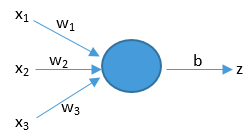
\includegraphics[width=8cm, height=3cm]{pictures/逻辑回归/1nn}
	\caption{线性回归}
	\label{fig:1nn}
\end{figure}

\subsection{激活函数-非线性预测结果}
\textbf{激活函数作用:预测结果,非线性,既有突变性,类似于神将元的突触,真正提高神经网络智商的函数。}
线性回归 + sigmoid激活函数 = 逻辑回归
在实际的神经网络中,我们不能直接使用线性回归,必须在逻辑回归外面加一个激活函数,如果没有它,神经网络永远智商高不起来,激活函数种类很多,这里介绍sigmoid函数。
\begin{equation}
	\bm{y' = \sigma (Z) = \frac{1}{1 + e^{-Z}}} \label{eq:sigmoid}
\end{equation}
公式\ref{eq:sigmoid}对应的图像如图\ref{fig:sigmoid}所示。

\begin{figure}[htb]
	\centering
	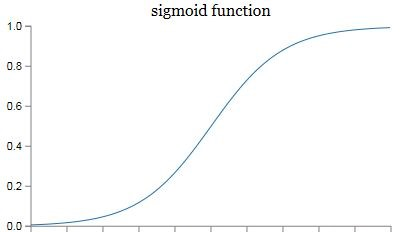
\includegraphics[width=0.7\linewidth]{pictures/激活函数/sigmoid}
	\caption{激活函数}
	\label{fig:sigmoid}
\end{figure}

sigmoid函数的一个作用就是把$z$映射到$[0, 1]$之间,上图的横坐标是$z$,纵坐标用$y'$表示,$y'$就代表了最终的预测结果,从图像中可以看出,$z$越大,$y'$就越靠近1,$z$越小,$y'$就越靠近0,把预测结果映射到$[0, 1]$,有利于神经网络的计算,也便于人类进行理解,在预测猫的例子中,如果$y'$是0.8,就说明有80\%的概率是猫。

\subsubsection{解释与说明}
\underline{逻辑回归返回的是概率,例如,用户点击“广告”的的概率是0.00023,也可以将概率转化为二元值,例如,这封电子邮件是垃圾邮件。}
逻辑回归(Logistic Regression)虽然被称为回归,但其实际上是分类模型,并常用于二分类。逻辑回归函数特点:简单、可并行化、可解释性强,深受工业界喜爱。逻辑回归函数属于广义线性模型,这一类模型形式基本都差不多,都具有$dot(w, x) + b$的形式,逻辑回归可以是二分类,也可以是多分类,但是二分类的更为常用,所以实际中使用的是二分类的逻辑回归。

\subsection{损失函数-预测与实际的差距}
\textbf{损失函数作用:判断单个训练样本的预测结果与实际结果的差距}

先回顾一下先前的预测算法,如下:	
\begin{align*}
	Z^{(i)} &= w^Tx^{(i)} + b \\
	\hat{y}^{(i)} &= \sigma (Z^{(i)}) = \frac{1}{1 + e^{-Z^{(i)}}}
\end{align*}

其中$\hat{y}$是预测结果,角标$i$指代第$i$个训练样本,$\hat{y}^{(i)}$是对于训练样本$x^{(i)}$的预测结果。
$$\bm{L(\hat{y}^{(i)}, y^{(i)}) = \frac{1}{2}(\hat{y}^{(i)} - y^{(i)})^2}$$

损失函数运算后的结果越大,那么预测就与实际结果的偏差越大,即预测精度越低。理论上可以用上面的公式作为损失函数--预测结果与实际结果的差的平方再乘以二分之一。但是在实践中通常不使用它,而是使用公式\ref{eq:loss_function}:
\begin{equation}
	\bm{L(\hat{y}^{(i)}, y^{(i)}) = -(y^{(i)}log(\hat{y}^{(i)}) + (1 - y^{(i)})log(1 - \hat{y}^{(i)}))} \label{eq:loss_function}
\end{equation}

这个新的损失函数作用与之前相同,努力使损失函数的值越小,就是努力让预测的结果越准确。

\subsubsection{解释与说明}
公式\ref{eq:loss_function}中的log(t)是python中的函数,实际上是以e为底的对数$\log_at$,也就是\bm{$\ln t$}。

\subsection{成本函数-预测与实际的差距}
\textbf{成本函数作用:判断整个训练集的预测结果与实际结果的差距}

损失函数是针对单个训练样本来定义的,成本函数是用来衡量整个训练集的预测精度。其实就是对每个训练样本的“损失”进行累加,然后求平均值。成本函数的公式如下:
\begin{equation}
	\bm{J(w,b) = \frac{1}{m}\sum_{i=1}^{m}L(\hat{y}^{(i)}, y^{(i)}) = - \frac{1}{m}\sum_{i=1}^{m}[(y^{(i)}log(\hat{y}^{(i)}) + (1 - y^{(i)})log(1 - \hat{y}^{(i)}))]} \label{eq:cost}
\end{equation}

损失函数定义:将随机事件或有关随机变量的取值映射为非负实数以表示该随机事件的风险或损失的函数。

损失函数的作用就是衡量模型预测的好坏,换一种说法就是衡量两个分布之间的距离:其中一个分布是原始分布,或者正确的分布,而另一个分布则是目前的分布,或者模型拟合的分布。

\subsection{梯度下降法-神经网络的学习功能}
\textbf{梯度下降法作用:预测是否准确由成本函数确定,而成本函数由权重w和阈值b影响,梯度下降法就是为了找出合适的w和b,一步步的调整w和b,新的w和b会使成本函数的输出结果更小,进一步让预测结果更加准确。}

回顾逻辑回归算法和损失函数,结合下面几个公式,输入x和实际结果y都是固定的,所以损失函数是一个关于w和b的函数,所谓“学习”或“训练神经网络”,就是找到一组w和b,使损失函数最小。

\begin{align*}
Z^{(i)} &= w^Tx^{(i)} + b \\
\hat{y}^{(i)} &= \sigma (Z^{(i)}) = \frac{1}{1 + e^{-Z^{(i)}}}
\end{align*}
 $$
\bm{J(w,b) = \frac{1}{m}\sum_{i=1}^{m}L(\hat{y}^{(i)}, y^{(i)}) = - \frac{1}{m}\sum_{i=1}^{m}[(y^{(i)}log(\hat{y}^{(i)}) + (1 - y^{(i)})log(1 - \hat{y}^{(i)}))]}
$$

\begin{figure}[htb]
	\centering
	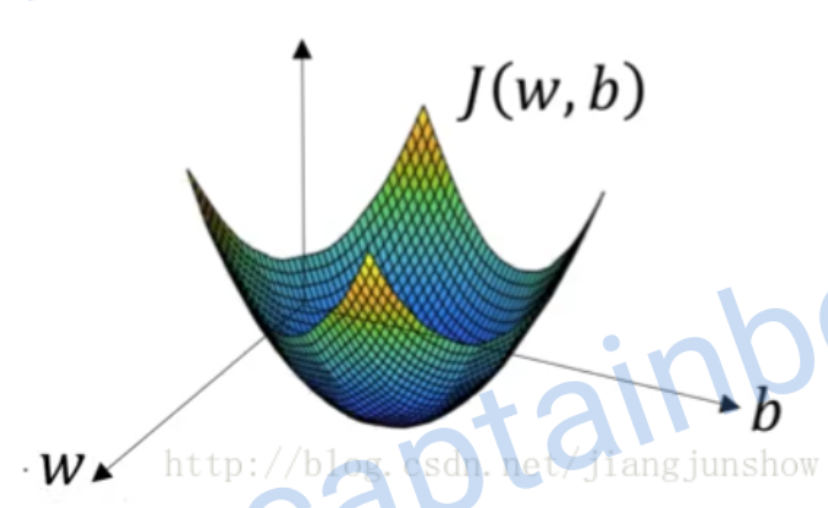
\includegraphics[width=0.7\linewidth]{pictures/成本/lost}
	\caption{损失函数}
	\label{fig:lost}
\end{figure}

如图\ref{fig:lost}所示,损失函数$J$的形状是一个漏斗状,我们训练的目标就是找到漏斗底部的一组$w$和$b$,这种漏斗状的函数被称为凸函数(这里指的是向下凸),我们选择公式\ref{eq:loss_function}作为损失函数的真正原因正是因为它是一个凸函数。

\begin{figure}[htb]
	\centering
	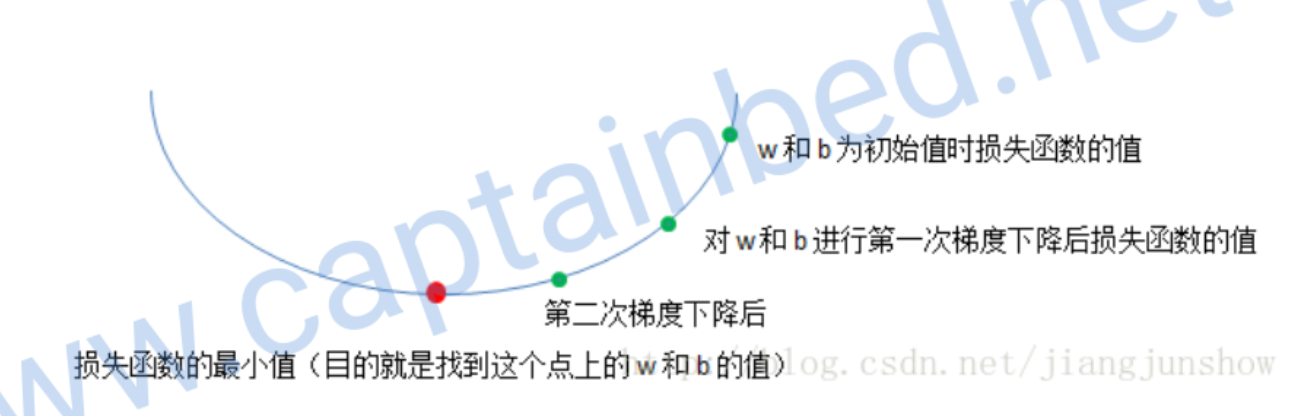
\includegraphics[width=0.7\linewidth]{pictures/梯度下降法/gradient_descent1}
	\caption{梯度下降过程}
	\label{fig:gradient_descent1}
\end{figure}

如图\ref{fig:gradient_descent1}所示,梯度下降法会一步步地更新$w$和$b$,使损失函数一步步地变小,最终找到最小值或接近最小值的地方。
\begin{figure}[htb]
	\centering
	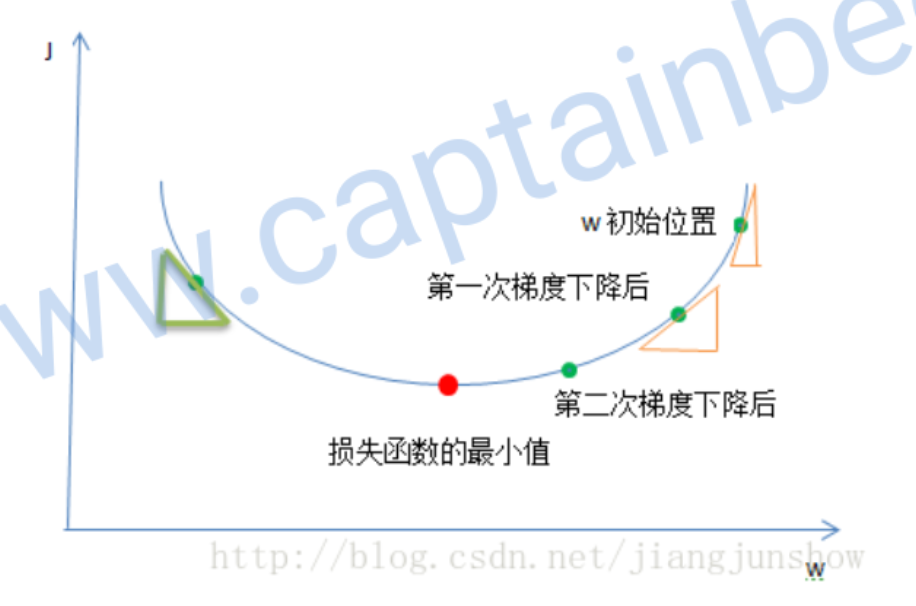
\includegraphics[width=0.7\linewidth]{pictures/梯度下降法/gradient_descent2}
	\caption{$J$关于$w$的梯度下降}
	\label{fig:gradient_descent2}
\end{figure}

为了简化问题,先假设损失函数$J$只有一个参数$w$,并且假设$w$只是一个实数(实际上$w$是一个向量)。如图\ref{fig:gradient_descent2}所示,梯度下降算法一步步改变着$w$的值,使损失函数的结果越来越小。
\begin{equation}
	\bm{w' = w - r * \frac{dJ}{dw}} \label{eq:gradient_descent}
\end{equation}
这里的$\frac{dJ}{dw}$就是图\ref{fig:gradient_descent2}中的斜率,这里的$w'$是下一次$w$的值(注意,这里$w'$不是导数),假定$\Delta w = w - w'$,那么公式\ref{eq:gradient_descent}可以转化为$\Delta w = r * \frac{dJ}{dw}$。

为简化起见,在床长人工智能教程中,$\textcolor{red}{\textbf{$\frac{dJ}{dw}$}}$省略写成$\textcolor{red}{\textbf{dw}}$,所以,公式\ref{eq:gradient_descent}可以写成如下形式:
\begin{equation}
	\textcolor{red}{\bm{w' = w - r * dw} \label{eq:gradient_descent2}}
\end{equation}

\subsubsection{解释与说明}
在梯度下降法中,有几点需要重点解释与说明一下:
\begin{enumerate}
	\item 损失函数为什么不选择平方差乘以$\frac{1}{2}$,而是采用公式\ref{eq:loss_function}的形式?
	损失函数的作用是为了获取预测结果与真实结果的差距,而梯度下降法是基于损失函数来迭代$w$和$b$,所以合理的损失函数能更好的计算梯度下降,基于公式\ref{eq:loss_function}得到的成本函数公式\ref{eq:cost}对$w$和$b$是凸函数,能更快速、更准确的得到$w$和$b$。所以\textcolor{red}{\textbf{选择合适的损失函数是为了更好的计算梯度下降。}}
	
	\item 梯度下降公式\ref{eq:gradient_descent2}中的\textcolor{red}{dw是$\frac{dJ}{dw}$的简写,$w'$不是导数,是$w$的下一次取值}。
	
	\item 梯度下降的学习率$r$实际上就是梯度下降前后两点的高度差$\Delta J$,很明显,在指定点$(w,J)$位置的斜率$\frac{dJ}{dw}$是个定值,高度差越大,$\Delta w$就越大。所以学习率$r$也是影响预测结果准确度的一个指标:
	如果学习率过小。学习周期(迭代次数)会很长,因为每次$\Delta w$变化很小;倘若成本函数存在多个凸点,可能会导致$w$进入局部最小而无法到达全局最小。
	如果学习率过大,可能会导致$w$跳过最小值,无法到达最小值,导致预测结果不准确。
	所以,选择合适的学习率很重要,一般学习率开始较大,然后逐渐衰减的过程。
	
	\item 为什么采用梯度下降法,而不是直接求$\frac{dJ}{dw} = 0$,找出此时的$w$呢?
	这里给出可能的原因:求出成本函数$J$的导数$\frac{dJ}{dw}$后,令其等于0,$\frac{dJ}{dw} = 0$,但是$w$往往不是一个参数,而是一个向量,有多少个输入特征,$w$就有多少个元素,一张普通的图片就有12288个特征呢,求12288个方程的解,采用高斯方程,矩阵的规模是12288 $\times$ 12288,求它的逆矩阵比较困难,甚至它不一定有逆矩阵。这就是为什么采用梯度下降法的原因。
\end{enumerate}

\subsection{神经网络的计算} 
	人工智能学习任务的核心就是模型的定义以及模型的参数求解方法。
	
	神经网络的计算是由一个前向传播及一个反向传播构成的。先通过前向传播计算出预测结果及损失;然后再通过反向传播计算出损失函数关于每一个参数$(w, b)$的偏导数,并对这些参数进行梯度下降,然后用新的参数进行新一轮的前向传播计算,这样来回不停的进行前向传播和反向传播计算来训练(更新)参数,使损失函数越来越小,使预测越来越精准。
	
\subsubsection{前向计算}
先回顾一下之前的几个公式:
\begin{align*}
Z^{(i)} &= w^Tx^{(i)} + b \\
\hat{y}^{(i)} &= \sigma (Z^{(i)}) = \frac{1}{1 + e^{-Z^{(i)}}} \\
L(\hat{y}^{(i)}, y^{(i)}) &= -(y^{(i)}log(\hat{y}^{(i)}) + (1 - y^{(i)})log(1 - \hat{y}^{(i)}))
\end{align*}
前向计算步骤:
\begin{enumerate}
	\item 给定初始值w和b以及输入值$x^{(i)}$(第$i$个训练样本,以及逻辑回归函数,得到$Z^{(i)}$;
	\item 根据$Z^{(i)}$和sigmoid激活函数,得到$\hat{y}^{(i)}$,也就是预测结果;
	\item 根据$\hat{y}^{(i)}$、$y^{(i)}$和损失函数$J$,得到第$i$个训练样本的预测结果和真实结果之间的差距。
\end{enumerate}

\subsubsection{反向计算}
反向计算分为两个步骤,先计算偏导数$\frac{dJ}{dw}$和$\frac{dJ}{db}$;根据梯度下降法$w' = w - r \times \frac{dJ}{dw}$和$b' = b - r \times \frac{dJ}{db}$来更新$w$和$b$的值。先将之前的公式罗列出来:
\begin{align*}
	z &= w^Tx + b \\
	a &= \hat{y} = \sigma (z) = \frac{1}{1 + e^{-z}} \\
	L(a, y) &= 	L(\hat{y}, y) = -(ylog(a) + (1 - y)log(1 - a))
\end{align*}

在给定输入特征$x$和真实结果$y$的条件下,损失函数$L(\hat{y}, y)$实际上是关于$w$和$b$的函数,$L(w, b)$是以上三个函数的复合函数,自变量变成了$w$和$b$了,因为$x$是输入的训练样本,为已知,对复合函数的求导就很简单了。
\begin{align}
\frac{dL}{dw} &= \frac{dL}{da} \times \frac{da}{dz} \times \frac{dz}{dw} \\
\frac{dL}{db} &= \frac{dL}{da} \times \frac{da}{dz} \times \frac{dz}{db}
\end{align}

\textcolor{red}{偏导数计算过程:}
\begin{enumerate}
	\item 计算$\frac{dL}{da}$。
		\begin{align*}
				L(a, y) &= 	L(\hat{y}, y) = -(ylog(a) + (1 - y)log(1 - a)) \\
				\frac{dL}{da} &=-\frac{y}{a} + \frac{1 - y}{1 - a}	
		\end{align*}
	
	\item 计算$\frac{da}{dz}$。
	\begin{align*}
		a = \hat{y} = \sigma (z) &= \frac{1}{1 + e^{-z}} \\
									a	&=\frac{e^z}{e^z + 1} \\
			 			\frac{da}{dz} &= \frac{e^z(e^z + 1) - e^{2z}}{(e^z + 1)^2} \\
			 								&= \frac{e^z}{(e^z + 1)^2}  \\
			 								&= \frac{a}{e^z + 1} \\
			 								&= \frac{a}{e^z + 1} - a + a\\
			 								&= a \times  (\frac{1}{e^z + 1} - 1) + a\\
			 								&= a \times (-a) + a \\
			 								&= a(1 	- a)
	\end{align*}

	\item 计算$\frac{dz}{dw}$。
	\begin{align*}
		z &= w \cdotp x + b \\
		\frac{dz}{dw} &= x
	\end{align*}
	
	
	\item 计算$\frac{dz}{db}$
	\begin{align*}
	z &= w \cdotp x + b \\
	\frac{dz}{db} &= 1
	\end{align*}
\end{enumerate}

各项偏导数公式如下:
\begin{equation}
	\frac{dL}{da} =-\frac{y}{a} + \frac{1 - y}{1 - a} \label{eq:derivative_loss}
\end{equation}

\begin{equation}
	\frac{da}{dz} =a(1 	- a) \label{eq:derivative_active}
\end{equation}

\begin{equation}
	\frac{dz}{dw} = x \label{eq:derivative_logistic_dw}
\end{equation}

\begin{equation}
	\frac{dz}{db} = 1 \label{eq:derivative_logistic_db}
\end{equation}

根据上面公式可知,只有逻辑回归函数涉及到w和b变量,中间函数不涉及到w和b,所以将$\frac{dL}{da} \times \frac{da}{dz}$整合成一个公式。注意,这里的a就是$\hat{y}$,是预测结果。
\begin{align*}
	\frac{dL}{dz} = \frac{dL}{da} \times \frac{da}{dz}  &= (-\frac{y}{a} + \frac{1 - y}{1 - a}) \times a(1 	- a) \\
	      																		&= y(a - 1) + a(1 - y) \\
	      																		&= a - y
\end{align*}

所以,最终神经网络的偏导数公式如下:
\begin{align*}
	\frac{dL}{dw} &= \frac{dL}{dz} \times \frac{dz}{dw} \\
						 &= \frac{dL}{dz} \times x \\
						 &= x(a-y)
\end{align*}

\begin{align*}
	\frac{dL}{db} &= \frac{dL}{dz} \times \frac{dz}{db} \\
						 &= \frac{dL}{dz} \times 1 \\
						 &= a-y
\end{align*}

最后根据梯度下降法$w' = w - r \times \frac{dL}{dw}$和$b' = b - r \times \frac{dL}{db}$来更新w和b。

\textbf{上面讲述的是单个训练样本的神经网络计算,多个训练样本的神经网络如何计算呢?}我们知道损失函数$L^{(i)}(w^{(i)},b^{(i)})$是单个训练样本的预测结果和实际结果的差距,成本函数是m组训练样本的平均值。
\begin{align*}
	J(w,b) = \frac{1}{m}\sum_{i=1}^{m}L(\hat{y}^{(i)}, y^{(i)}) &= \frac{1}{m}\sum_{i=1}^{m}L^{(i)}(w^{(i)},b^{(i)}) \\
	\frac{dJ}{dw} &= \frac{1}{m}\sum_{i=1}^{m}\frac{dL^{(i)}}{dw^{(i)}} \\
	\frac{dJ}{db} &= \frac{1}{m}\sum_{i=1}^{m}\frac{dL^{(i)}}{db^{(i)}}
\end{align*}

所以,\textcolor{red}{\textbf{多个样本时的偏导数等于每个样本的偏导数的平均值,}}不要把事情弄复杂。

\subsubsection{解释与说明}
上面这些公式都是针对与特定的函数来说的,因为在不同的神经网络中,会有不同的逻辑回归函数、不同的激活函数、不同的损失函数等,得到的公式、偏导数会有差异,但是计算流程是相似的。

单就损失函数来说,损失函数就有Zero-one Loss(0-1损失),Perceptron Loss(感知损失),Hinge Loss(铰链损失),CrossEntropyLoss(交叉熵损失函数)等等。

\subsection{向量化}
向量化对人工智能编程是非常重要的,因为训练一个模型需要非常多的数据,也就是说计算量非常大,需要很长的计算时间,向量化可以大大提升计算速度(可节约高达300倍时间)。对于一张64$\times$64图片有12288个特征。
前向计算的逻辑回归函数中,每一个特征和一个权重相乘,需要执行12288次乘法,如果训练样本达到$10^9$,那么乘法次数达到$12288\times 10^9$次,后续还有激活函数、损失函数的计算等等;另外还有反向计算,如果再迭代很多次,计算量大的无法估量。假定两个矩阵相乘$RES_{m\times h} = W_{m\times n}\cdot X_{n\times h}$,在python中,如果采用3层for循环计算,代码如下:
\begin{lstlisting}[{language=Python}]
for i in range(0, m):
	for j in range(0, h):
		for k in range(0, n):
			RES[i,j] += W[i, k] * X[k, j]	
\end{lstlisting}

乘法的计算量为$m\cdot n \cdot h$,如果单纯通过for循环实现,for循环代码在一个线程中运行,计算量会很大,同时,由于python是解释性语言,每执行一次for循环,就要解释一次并调用c代码,就更慢了。
如果采用numpy中的向量点乘运算,首先,代码会十分简洁,其次,解释次数会减少,最后,矩阵W第i行与矩阵X第j列相乘和矩阵W第i+1行与矩阵X第j+1列相乘,从计算上来讲是独立的,所以,numpy的向量点乘底层可能是采用多线程实现,每一条计算作为独立的一个任务,大大提高了运算效率。具体代码如下:
\begin{lstlisting}[language=Python]
import numpy as np

RES = np.dot(W, X)
\end{lstlisting}

另外,现在的计算机大部分都是SIMD(单指令多数据流),如果使用for循环的话,那么一条指令的数据流就是for循环里面规定的,并没有进行并行运算,没有充分利用计算机资源,\textcolor{red}{\textbf{所以在深度学习里面,使用显示的循环会让运算速度十分的缓慢,要尽量用向量化取代循环代码,向量化是非常基础的去除代码中for循环的艺术。}}

\subsection{基础概念}
学习了人工智能的基础知识后,下面对一些基础概念做一下汇总。
\begin{itemize}
	\item \textbf{标签} \\
	标签是我们要预测的事物,即简单线性回归中的y变量。标签可以是小麦未来的价格、图片中显示的动物品种、音频剪辑的含义或任何事物。
	\item \textbf{特征}  \\
	特征是输入变量,即简单线性回归中的x变量。简单的机器学习项目可能会使用单个特征,而比较复杂机器学习项目可能会使用上百万个特征。
	在垃圾邮件人工智能检测器中,特征可能包括:电子邮件文本中的字词,发件人的地址,发送电子邮件的时段等。
	\item \textbf{样本} \\
	样本是指数据的特定实例:x。我们将样本分为两类:有标签样本和无标签样本。
	有标签样本同时包含特征和标签,即(x, y)。我们使用有标签样本来训练模型。在垃圾邮件检测器中,有标签样本是用户明确标记为“垃圾邮件”和“非垃圾邮件”的各个电子邮件。
	无标签样本包含特征,但是不包含标签。即(x, ?)。在使用有标签样本训练模型之后,我们会使用该模型来预测无标签样本的标签。在垃圾邮件检测器中,无标签样本是用户尚未添加标签的新电子邮件。
	\item \textbf{模型} \\
	模型定义了特征与标签之间的关系。垃圾邮件检测模型可能会将某些特征与“垃圾邮件”紧密联系起来,关于模型生命周期的两个阶段:
	训练是指创建或学习模型。向模型展示有标签样本,让模型逐渐学习特征与标签之间的关系。
	推断是指将训练后的模型应用于无标签样本。使用经过训练的模型做出有用的预测($y'$)。
\end{itemize}

\subsection{特征工程-将原始信息转为特征矢量}
\textbf{神经网络的输入特征矢量是如何来的呢?} 
机器学习模型一般都需要将特征表示为实数向量,因为特征值要与模型权重相乘。
\begin{figure}
	\centering
	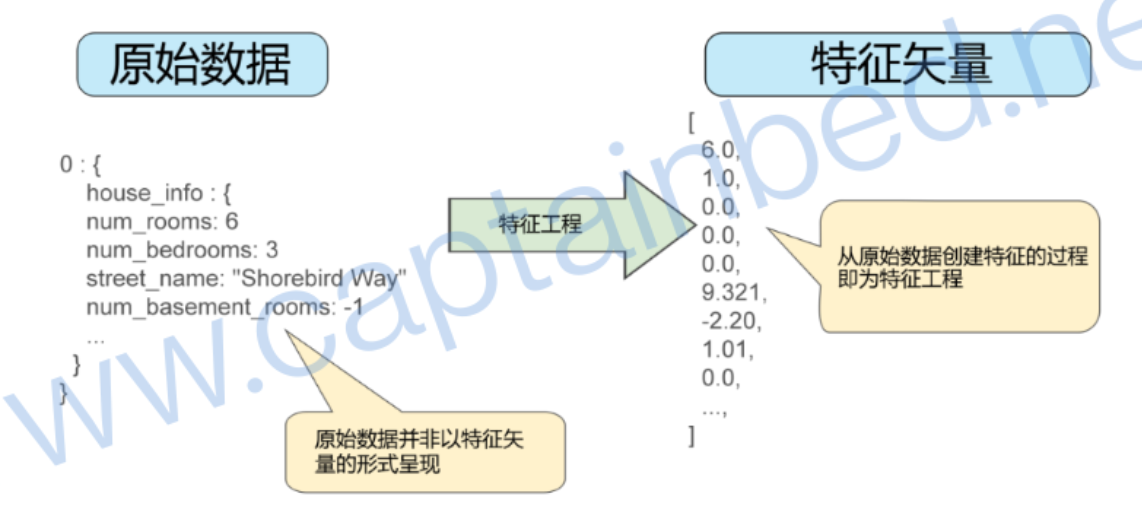
\includegraphics[width=0.7\linewidth]{pictures/特征工程/vector1}
	\caption{}
	\label{fig:vector1}
\end{figure}
对于图片模型,它的特征矢量我们很清楚是什么,它的每个特征都是一个颜色值。但是有些模型的特征值不是数值,而是字符串或是其他无法用数值表示的信息时,会变得比较棘手。我们可以采用分类特征的方法来解决这一问题。

\textbf{分类特征的重要思想}:
\begin{itemize}
	\item 关键思想之一就是\textbf{定义一个从特征值到整数的映射。}  \\
		举例说明,假定我们有一个特征city\_name,用来表示城市名字,它的值可能是“北京”、“上海”、“深圳”,由于模型不能将字符串与学习到的权重相乘,因此我们需要使用特征工程将字符串转化为数值,要实现这一点,需要定义一个从特征值到整数的映射,世界上的每个城市并非都会出现在我们的数据集中,那些没有出现在数据库中的其他城市划分为“其他”类别。
		我们可以按照上面方法将“北京”映射为1,“上海”映射为2,“深圳”映射为3,“其他”映射为4。
		这样就可以实现特征值和权重的相乘了。
	\item 关键思想之二就是\textbf{独热编码和多热编码} \\
	 	本来“北京”、“上海”、“深圳”、“其他”只是城市的名字,没有先后顺序之分,但是上面强行给了一个顺序,显然是不合理的。   \\
	 	独热编码(One-Hot Encoding),又称一位有效编码,其方法是使用N位状态寄存器来对N个状态进行编码,每个状态都有它独立的寄存器位,并且在任意时候,其中只有一位有效。即,只有一位是1,其余都是零值。
	 	假定我们只有4中状态,按照独热编码,我们可以将“北京”映射为0001,“上海”映射为0010,“深圳”映射为0100,“其他”映射为1000。     \\
	 	\textbf{为什么要进行独热编码?}
	 	在回归,分类,聚类等机器学习算法中,特征之间距离的计算或相似度的计算是非常重要的。而常用的距离或相似度的计算都是在欧式空间的相似度计算,计算余弦相似性,基于的就是欧式空间。
	 	使用独热编码(One-Hot Encoding),将离散特征的取值扩展到了欧式空间,离散特征的某个取值就对应欧式空间的某个点。将离散型特征使用独热编码(One-Hot Encoding),会让特征之间的距离计算更加合理。
	 	比如上面的城市名特征,该离散型特征,共有4个取值,不使用独热编码(One-Hot Encoding),两个城市名之间的距离:
	 	d(北京,上海) = 1 \\
	 	d(北京,深圳) = 2 \\
	 	d(北京,其他) = 3 \\
	 	$\hdots$  \\
	 	实际上,这里只是城市名之间的距离,或者换成一个人的工作职业,每个工作职业之间的距离应该都是相同的,而不应该是随着映射的不同而不同。\\
	 	使用独热编码之后,两个城市名之间的距离都是$\sqrt{2}$,即每两个城市名之间的距离都是一样的,显得合理。\\
	 	多热编码,指的是有多位有效编码,可能有多位为1。举例,一个人可能有多个工作职业,假定职业有4种状态,“厨师”、“演员”、“老师”、“歌手”,一个人可能既是演员又是歌手,所以她的编码可能是0101,存在2个有效位。
\end{itemize}

\textbf{分类特征使用场景} \\
当特征值存在分类时,需要做映射,如果特征值不存在先后顺序,需要做独热编码或多热编码,如果特征值的数据本身特定含义,不需要做特征映射和独热编码等。


\subsection{深度学习注意事项}
\begin{itemize}
	\item 特征缩放 \\
	对输入特征进行特征缩放,受益的梯度下降效率和准确度
	\item 向量化
	对代码做向量化,提高计算效率
	\item 特征工程
	对输入特征进行处理,方便特征值和权重相乘
	\item 合适的损失函数
	选择合适的损失函数,方便成本函数关于w和b为凸函数
\end{itemize}